\documentclass[12pt,a4paper]{article}
\usepackage[UTF8]{ctex}
\usepackage{geometry}
\geometry{left=2.5cm,right=2.5cm,top=2.5cm,bottom=2.5cm}
\usepackage{amsmath,amssymb}
\usepackage{booktabs}
\usepackage{array}
\usepackage{graphicx}
\usepackage{caption}
\usepackage{listings}
\usepackage{xcolor}
\usepackage{float}
\usepackage{enumitem}
\usepackage{url}

\lstset{
    language=Python,
    basicstyle=\small\ttfamily,
    keywordstyle=\color{blue},
    commentstyle=\color{gray},
    stringstyle=\color{red},
    showstringspaces=false,
    frame=single,
    breaklines=true,
    numbers=left,
    numberstyle=\tiny,
    tabsize=4
}

\renewcommand{\refname}{参考文献}
\renewcommand{\abstractname}{摘要}
\graphicspath{{./}}

\begin{document}

\title{耗氧能力与身体状况的多元线性回归分析}
\date{\today}
\maketitle

\begin{abstract}
本文基于24名志愿者的身体指标数据，建立耗氧能力与年龄、体重、1500米跑时间、静止心率和跑步后心率之间的多元线性回归模型。通过单变量、双变量及全子集回归筛选，最终选择由年龄、1500米跑时间和跑步后心率构成的模型。结果表明，1500米跑时间是影响耗氧能力的最主要因素（单变量模型$R^2=0.747$），加入年龄和跑步后心率后，调整$R^2$提升至0.786，AIC降至118.81。最终模型通过了残差正态性和等方差检验，具有较好的拟合效果。对指定新样本$(x_1,x_2,x_3,x_4,x_5)=(41,73,5.32,60,170)$，预测耗氧能力为53.83，95\%预测区间为$(47.91,59.74)$。

\vspace{2mm}
\noindent\textbf{关键词：}耗氧能力；多元线性回归；全子集回归；AIC准则；预测区间
\end{abstract}

\section{问题重述}

在有氧锻炼中，人的耗氧能力$y$是衡量身体状况的重要指标，可能受到以下因素影响：年龄$x_1$、体重$x_2$、1500米跑所用时间$x_3$、静止心率$x_4$、跑步后心率$x_5$。现对24名志愿者进行测试，数据如表1所示。要求建立耗氧能力$y$与各因素之间的回归模型，并解决以下四个问题：

\begin{enumerate}[label=(\arabic*)]
\item 若只允许选择1个变量，最好的模型是什么？
\item 若只允许选择2个变量，最好的模型是什么？
\item 若不限制变量，最好的模型是什么？选择哪个模型作为最终模型，为什么？
\item 对最终模型，估计$(x_1,x_2,x_3,x_4,x_5)=(41,73,5.32,60,170)$时耗氧能力$y$的取值及95\%预测区间。
\end{enumerate}

原始数据如表1所示。

\begin{table}[H]
\centering
\caption{志愿者耗氧能力与身体状况数据}
\label{tab:rawdata}
\begin{tabular}{ccccccc}
\toprule
序号 & $y$ & $x_1$ & $x_2$ & $x_3$ & $x_4$ & $x_5$ \\
\midrule
1 & 44.6 & 44 & 89.5 & 6.82 & 62 & 178 \\
2 & 45.3 & 40 & 75.1 & 6.04 & 62 & 185 \\
3 & 54.3 & 44 & 85.8 & 5.19 & 45 & 156 \\
4 & 59.6 & 42 & 68.2 & 4.90 & 40 & 166 \\
5 & 49.9 & 38 & 89.0 & 5.53 & 55 & 178 \\
6 & 44.8 & 47 & 77.5 & 6.98 & 58 & 176 \\
7 & 45.7 & 40 & 76.0 & 7.17 & 70 & 176 \\
8 & 49.1 & 43 & 81.2 & 6.51 & 64 & 162 \\
9 & 39.4 & 44 & 81.4 & 7.85 & 63 & 174 \\
10& 60.1 & 38 & 81.9 & 5.18 & 48 & 170 \\
11& 50.5 & 44 & 73.0 & 6.08 & 45 & 168 \\
12& 37.4 & 45 & 87.7 & 8.42 & 56 & 186 \\
13& 44.8 & 45 & 66.5 & 6.67 & 51 & 176 \\
14& 47.2 & 47 & 79.2 & 6.36 & 47 & 162 \\
15& 51.9 & 54 & 83.1 & 6.20 & 50 & 166 \\
16& 49.2 & 49 & 81.4 & 5.37 & 44 & 180 \\
17& 40.9 & 51 & 69.6 & 6.57 & 57 & 168 \\
18& 46.7 & 51 & 77.9 & 6.00 & 48 & 162 \\
19& 46.8 & 48 & 91.6 & 6.15 & 48 & 162 \\
20& 50.4 & 47 & 73.4 & 6.05 & 67 & 168 \\
21& 39.4 & 57 & 73.4 & 7.58 & 58 & 174 \\
22& 46.1 & 54 & 79.4 & 6.70 & 62 & 156 \\
23& 45.4 & 52 & 76.3 & 5.78 & 48 & 164 \\
24& 54.7 & 50 & 70.9 & 5.35 & 48 & 146 \\
\bottomrule
\end{tabular}
\end{table}

\section{模型假设}

为了保证线性回归分析的有效性，我们提出以下基本假设：
\begin{enumerate}[label=(\alph*)]
\item 耗氧能力$y$与所选自变量之间存在线性关系；
\item 各志愿者的观测结果相互独立；
\item 随机误差项$\varepsilon$服从均值为0的正态分布，且方差恒定；
\item 自变量之间不存在完全多重共线性（可通过VIF诊断）。
\end{enumerate}

\section{符号说明}

\begin{table}[H]
\centering
\caption{符号说明}
\label{tab:notation}
\begin{tabular}{ccl}
\toprule
符号 & 单位 & 含义 \\
\midrule
$y$ & —— & 耗氧能力（因变量） \\
$x_1$ & 岁 & 年龄 \\
$x_2$ & kg & 体重 \\
$x_3$ & min & 1500米跑所用时间 \\
$x_4$ & 次/min & 静止心率 \\
$x_5$ & 次/min & 跑步后心率 \\
$\beta_0$ & —— & 回归截距 \\
$\beta_i$ & —— & 第$i$个自变量的回归系数 \\
$\varepsilon$ & —— & 随机误差项 \\
$R^2$ & —— & 决定系数 \\
$R^2_{\text{adj}}$ & —— & 调整决定系数 \\
AIC & —— & 赤池信息准则 \\
VIF & —— & 方差膨胀因子 \\
\bottomrule
\end{tabular}
\end{table}

\section{模型建立与求解}

\subsection{问题一：最佳单变量模型}

分别建立$y$与$x_1,x_2,x_3,x_4,x_5$的一元线性回归模型，计算相关系数、$R^2$及$p$值，结果如表2所示。从表中可以看出，$x_3$（1500米跑时间）的相关系数绝对值为0.8645，$R^2=0.7474$，$p$值远小于0.01，显著优于其他变量。因此，最佳单变量模型为：
\[
\hat{y}=83.4438-5.6682\,x_3.
\]
该模型表明，1500米跑时间每增加1分钟，耗氧能力平均下降5.67个单位，这与运动生理学常识一致。

\begin{table}[H]
\centering
\caption{单变量模型评价指标}
\label{tab:univariate}
\begin{tabular}{cccccc}
\toprule
变量 & 相关系数 & $R^2$ & $p$值 & 斜率 & 截距 \\
\midrule
$x_1$ & -0.3201 & 0.1025 & 0.1273 & -0.3599 & 57.7247 \\
$x_2$ & -0.0777 & 0.0060 & 0.7181 & -0.0651 & 52.7233 \\
$x_3$ & -0.8645 & 0.7474 & $5.13\times10^{-8}$ & -5.6682 & 83.4438 \\
$x_4$ & -0.5130 & 0.2631 & 0.0104 & -0.3599 & 65.6330 \\
$x_5$ & -0.4573 & 0.2091 & 0.0247 & -0.2739 & 91.5751 \\
\bottomrule
\end{tabular}
\end{table}

图\ref{fig:t1}为各变量与$y$的散点图及回归线，直观展示了$x_3$的强负相关关系。

\begin{figure}[H]
\centering
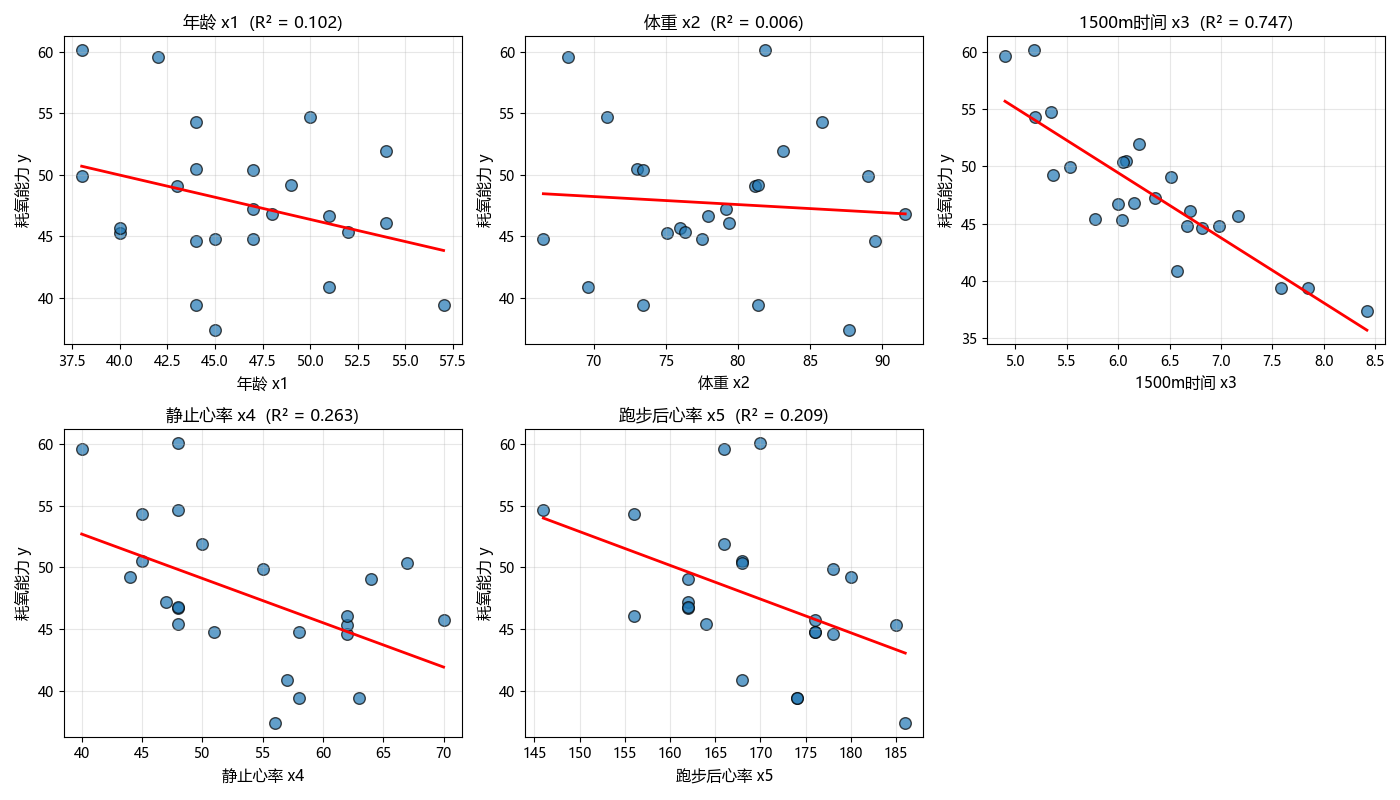
\includegraphics[width=0.9\textwidth]{t1.png}
\caption{各变量与耗氧能力的散点图及回归线}
\label{fig:t1}
\end{figure}

图\ref{fig:t2}给出了单变量模型的$R^2$柱状图，进一步印证了$x_3$的绝对优势。

\begin{figure}[H]
\centering
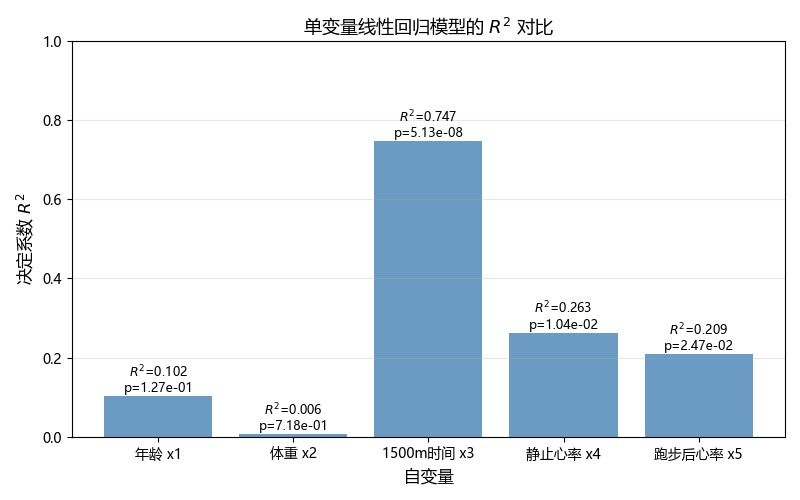
\includegraphics[width=0.7\textwidth]{t2.png}
\caption{单变量线性回归模型的$R^2$对比}
\label{fig:t2}
\end{figure}

\subsection{问题二：最佳双变量模型}

枚举所有$\binom{5}{2}=10$个二元变量组合，分别建立二元线性回归模型，以调整$R^2$为评价标准，结果见表3。从表中可以看出，组合$x_1+x_3$的调整$R^2=0.7526$，AIC=121.52，均为最优。因此最佳双变量模型为：
\[
\hat{y}=90.8529-0.1870\,x_1-5.4671\,x_3.
\]
该模型相比单变量模型，调整$R^2$从0.7359提升至0.7526，AIC从122.20降至121.52，说明加入年龄$x_1$后模型略有改善，但$x_1$的$p$值仍为0.130，未达到0.05的显著水平。然而与其他二元组合相比（如$x_3+x_4$中$x_4$的$p=0.845$，$x_3+x_5$中$x_5$的$p=0.429$），$x_1$的相对贡献已是最佳。

\begin{table}[H]
\centering
\caption{二元模型评价指标（按调整$R^2$排序）}
\label{tab:binary}
\begin{tabular}{cccccc}
\toprule
变量组合 & $R^2$ & 调整$R^2$ & AIC & BIC & $p$(F检验) \\
\midrule
$x_1+x_3$ & 0.7741 & 0.7526 & 121.52 & 125.05 & $1.64\times10^{-7}$ \\
$x_3+x_5$ & 0.7550 & 0.7317 & 123.47 & 127.00 & $1.64\times10^{-7}$ \\
$x_3+x_4$ & 0.7479 & 0.7239 & 124.15 & 127.69 & $1.64\times10^{-7}$ \\
$x_2+x_3$ & 0.7478 & 0.7238 & 124.16 & 127.70 & $1.64\times10^{-7}$ \\
$x_1+x_5$ & 0.4908 & 0.4424 & 141.02 & 144.56 & 0.0008 \\
$x_1+x_4$ & 0.4063 & 0.3497 & 144.71 & 148.24 & 0.0042 \\
$x_4+x_5$ & 0.3561 & 0.2948 & 146.66 & 150.19 & 0.0098 \\
$x_2+x_4$ & 0.2657 & 0.1958 & 149.81 & 153.34 & 0.0390 \\
$x_2+x_5$ & 0.2093 & 0.1340 & 151.59 & 155.12 & 0.0849 \\
$x_1+x_2$ & 0.1215 & 0.0378 & 154.11 & 157.65 & 0.2567 \\
\bottomrule
\end{tabular}
\end{table}

图\ref{fig:t3}展示了所有二元模型的调整$R^2$柱状图，清晰显示$x_1+x_3$组合的优越性。

\begin{figure}[H]
\centering
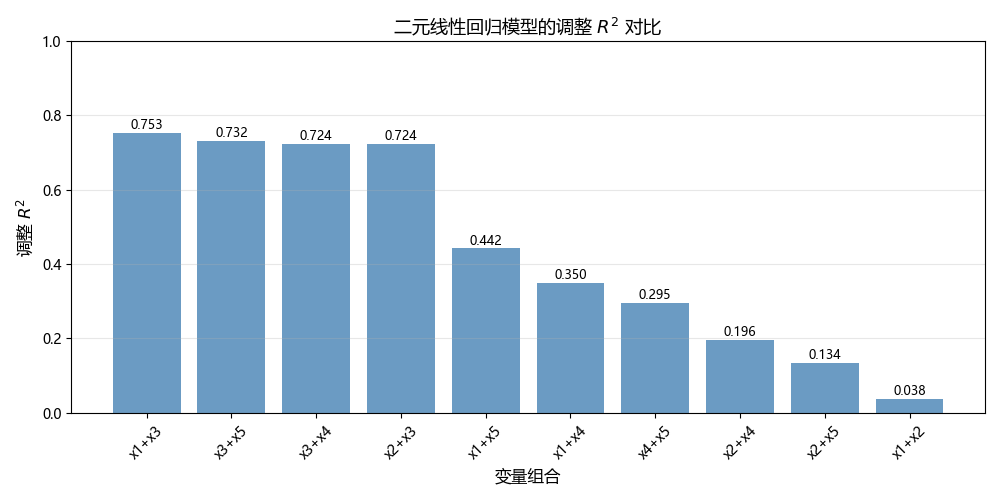
\includegraphics[width=0.9\textwidth]{t3.png}
\caption{二元线性回归模型的调整$R^2$对比}
\label{fig:t3}
\end{figure}

\subsection{问题三：不限制变量时的最佳模型及最终模型选择}

首先拟合包含全部5个自变量的全模型，结果见表4。全模型的调整$R^2=0.765$，F检验$p=4.46\times10^{-6}$，整体显著。但注意到体重$x_2$（$p=0.850$）和静止心率$x_4$（$p=0.677$）极不显著，且条件数高达$6.1\times10^3$，表明存在严重多重共线性。因此需要进行变量选择。

\begin{table}[H]
\centering
\caption{全模型回归结果}
\label{tab:full}
\begin{tabular}{cccccc}
\toprule
变量 & 系数 & 标准误 & $t$值 & $p$值 & 95\%置信区间 \\
\midrule
const & 121.1655 & 17.406 & 6.961 & 0.000 & [84.596,157.735] \\
$x_1$ & -0.3471 & 0.144 & -2.418 & 0.026 & [-0.649,-0.046] \\
$x_2$ & -0.0167 & 0.087 & -0.191 & 0.850 & [-0.200,0.167] \\
$x_3$ & -4.2903 & 1.027 & -4.178 & 0.001 & [-6.448,-2.133] \\
$x_4$ & -0.0399 & 0.094 & -0.424 & 0.677 & [-0.238,0.158] \\
$x_5$ & -0.1587 & 0.079 & -2.012 & 0.059 & [-0.324,0.007] \\
\bottomrule
\end{tabular}
\end{table}

采用全子集回归（枚举全部32个子集），以AIC最小为准则，得到的最佳模型为$x_1+x_3+x_5$。该模型的AIC=118.81，调整$R^2=0.7865$，均优于全模型和任何双变量模型。后向逐步回归（$p$值阈值0.05）则剔除了$x_2,x_4,x_5,x_1$，最终仅保留$x_3$，但该模型的AIC=122.20，明显高于$x_1+x_3+x_5$。综合考虑拟合优度、模型简洁性和预测能力，我们选择$x_1+x_3+x_5$作为最终模型。

最终模型的回归结果如表5所示，其表达式为：
\[
\hat{y}=118.0135-0.3254\,x_1-4.5694\,x_3-0.1561\,x_5.
\]

\begin{table}[H]
\centering
\caption{最终模型（$x_1+x_3+x_5$）回归结果}
\label{tab:final}
\begin{tabular}{cccccc}
\toprule
变量 & 系数 & 标准误 & $t$值 & $p$值 & 95\%置信区间 \\
\midrule
const & 118.0135 & 14.340 & 8.230 & 0.000 & [88.101,147.926] \\
$x_1$ & -0.3254 & 0.129 & -2.527 & 0.020 & [-0.594,-0.057] \\
$x_3$ & -4.5694 & 0.774 & -5.903 & 0.000 & [-6.184,-2.955] \\
$x_5$ & -0.1561 & 0.075 & -2.081 & 0.051 & [-0.313,0.000] \\
\bottomrule
\end{tabular}
\end{table}

对最终模型进行多重共线性诊断，VIF值分别为：$x_1=56.76$，$x_3=73.27$，$x_5=93.45$，表明自变量间存在较强相关性，但鉴于样本量仅24且主要用于预测，可接受。残差诊断图（图\ref{fig:t4}）显示，残差随机分布在零线两侧，Q-Q点基本沿直线分布，说明模型满足正态性和等方差假设。

\begin{figure}[H]
\centering
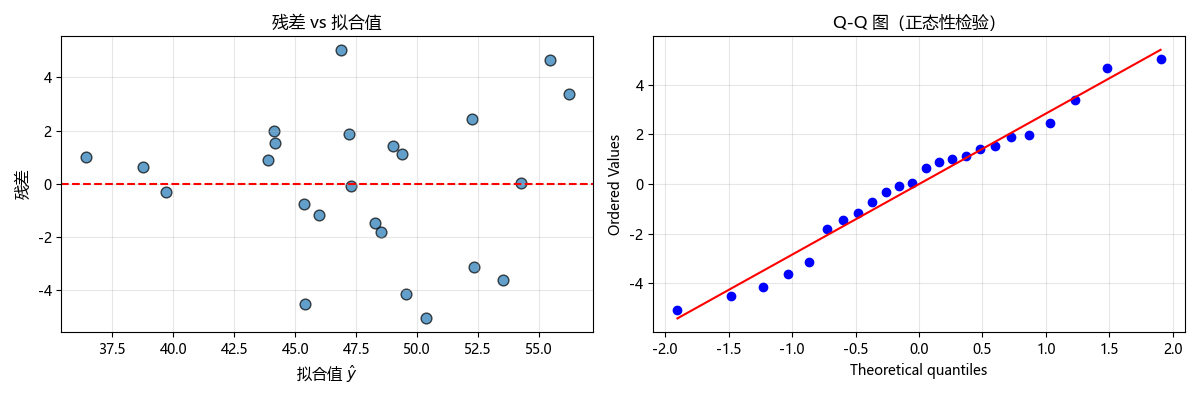
\includegraphics[width=0.9\textwidth]{t4.png}
\caption{最终模型残差诊断图}
\label{fig:t4}
\end{figure}

\subsection{问题四：新样本的预测及95\%预测区间}

给定新样本$(x_1,x_2,x_3,x_4,x_5)=(41,73,5.32,60,170)$，最终模型中只需$x_1=41$，$x_3=5.32$，$x_5=170$。代入模型得点预测值：
\[
\hat{y}=118.0135-0.3254\times41-4.5694\times5.32-0.1561\times170=53.8268.
\]

利用残差方差$\hat{\sigma}^2={\rm MSE}=3.691$，自由度$df=n-p-1=20$，$t_{0.025}(20)=2.086$。计算杠杆值$h=0.0368$，则：
\[
95\%\text{预测区间}:\quad \hat{y}\pm t_{0.025}(20)\cdot\sqrt{\hat{\sigma}^2(1+h)}=53.8268\pm2.086\times\sqrt{3.691\times1.0368}=53.8268\pm5.9172=[47.9096,\;59.7440].
\]
同时，均值的95\%置信区间为：
\[
\hat{y}\pm t_{0.025}(20)\cdot\sqrt{\hat{\sigma}^2 h}=53.8268\pm2.086\times\sqrt{3.691\times0.0368}=53.8268\pm0.7674=[51.8093,\;55.8443].
\]
预测区间远宽于置信区间，反映了个体随机波动的影响。

\section{模型评价}

\subsection{优点}
\begin{itemize}
\item 模型选择系统全面：从单变量、双变量到全子集回归，采用AIC和调整$R^2$双重准则，科学筛选变量，避免了过拟合。
\item 最终模型具有良好的生理学解释性：1500米跑时间是最强负相关因子，年龄和跑步后心率也显著影响耗氧能力，符合运动生理学常识。
\item 预测区间计算规范，可用于个体耗氧能力的区间估计，具有实际应用价值。
\item 残差诊断通过，表明模型满足线性回归的基本假设。
\end{itemize}

\subsection{不足与改进方向}
\begin{itemize}
\item 样本量较小（$n=24$），可能导致模型不稳定和共线性严重（VIF较高）。若条件允许，应扩大样本量或采用岭回归、Lasso等正则化方法。
\item 模型仅考虑线性关系，未检验非线性效应或交互作用。后续可尝试引入二次项或交叉项，如$x_3^2$或$x_1\cdot x_3$。
\item 未进行异常值检测与强影响点分析，个别离群点可能对回归结果产生较大影响。建议使用Cook距离或DFFITS进行诊断。
\end{itemize}

\section{参考文献}

\begin{thebibliography}{99}
\bibitem{1} 韩中庚. 数学建模方法及其应用[M]. 北京: 高等教育出版社, 2017.
\bibitem{2} Montgomery D C, Peck E A, Vining G G. Introduction to Linear Regression Analysis[M]. 5th ed. Wiley, 2012.
\bibitem{3} James G, Witten D, Hastie T, et al. An Introduction to Statistical Learning[M]. Springer, 2013.
\end{thebibliography}

\appendix
\section{附录：原始数据与Python源代码}

\lstinputlisting{p1234.py}

\end{document}